%!TEX root = p.tex
\section{Explorer   1}


\begin{figure}[htb]
  \centerline{
    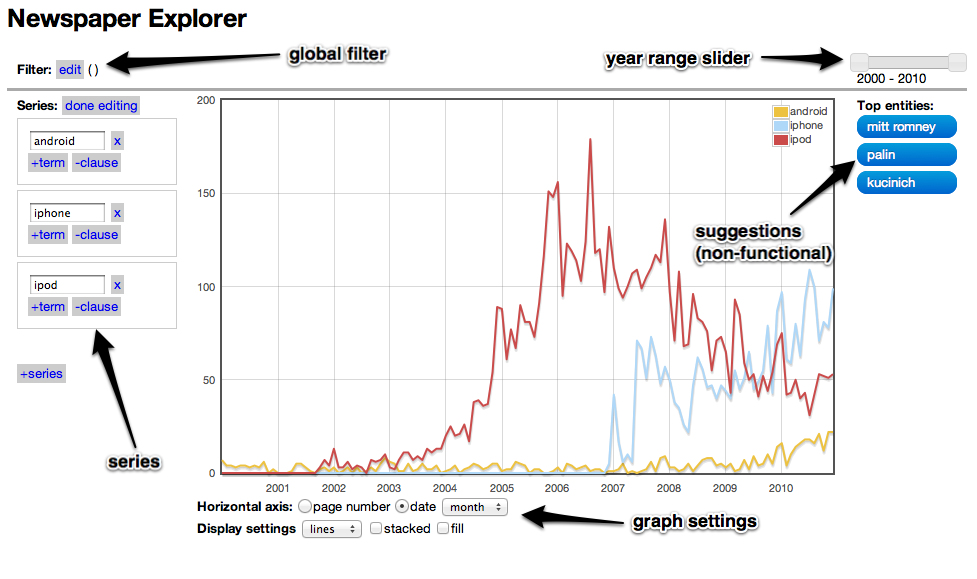
\includegraphics[scale=0.28]{figures/explorer-prototype.png}
  }
  \caption{TODO: FILL ME IN}
  \label{fig:explorer-prototype}
\end{figure}

The first iteration of the �Explorer� interface was designed to allow the visualization of the number of articles containing a given term, bucketed either by time or article page number. It borrowed the concept of �series� from Excel and other familiar charting tools, but allowed the specification of series as unions of the sets of documents containing specified words. For instance, a series like �dog OR cat� could be specified, and the series plotted would represent the number of documents containing one or both of these words. Additionally, this version allowed the user to specify a global filter, which would restrict the view to include only articles that match the series queries as well as the filter query. For instance, if one were to use �pet� as the filter and �dog� and �cat� as series, the two plot lines would represent the result of running queries for �pet AND dog� and �pet AND cat.� The version allowed the specification of arbitrary conjunctive normal form expressions for the filter. Beyond the series and filter features, this first iteration included a number of other features that are self-explanatory, including a year slider, numerous selection widgets for graph settings. 